\chapter{実装} \label{implementation}

\simname は Python を用いて実装されている。入力と表示に Jupyter Notebook~\cite{kluyver_jupyter_nodate} 、グラフの描画に matplotlib~\cite{hunter_matplotlib_2007} 、方程式の処理や数値計算に SymPy~\cite{meurer_sympy_2017} を用いている。

\section{使用している道具}

\subsection{Jupyter Notebook}
Jupyter Notebook は IPython~\cite{perez_ipython_2007} から分離したプロジェクトである。Jupyter Notebook から IPython カーネルを呼び出すことで、Python のコードを対話的に実行することができる。また、ipywidgets ライブラリを利用すると、Jupyter Notebook 上に GUI を作成することができる。図~\ref{example_jupyter}は、Jupyter Notebook 上にクリックすることのできる Button と、文字を入力できる Text の Widget を生成する例である。

\begin{figure}[htb]
\centering
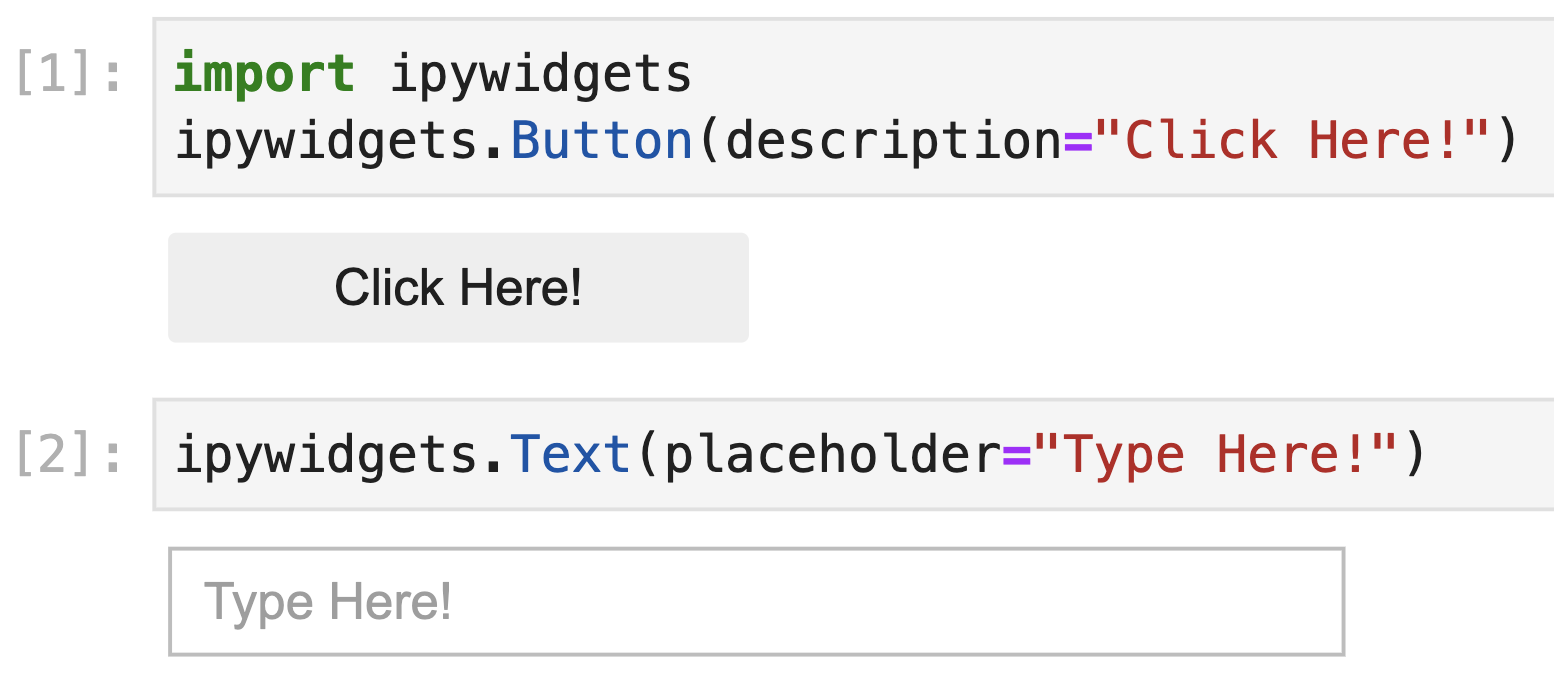
\includegraphics[width=0.9\linewidth]{work/example_jupyter.png}
\caption{Jupyter Notebook 上に Button と Text の
Widget を生成する例} \label{example_jupyter}
\end{figure}

\subsection{matplotlib}
matplotlib は、グラフを描画するためのライブラリである。Jupyter Notebook 上で matplotlib を用いると、グラフを Jupyter Notebook に表示することができる。また、出力先として ipywidgets の Output を用いることで、ipywidgets で作成した GUI にグラフを組み込むことができる。図~\ref{example_matplotlib} は matplotlib を用いて簡単なグラフを描画する例である。

\begin{figure}[htb]
\centering
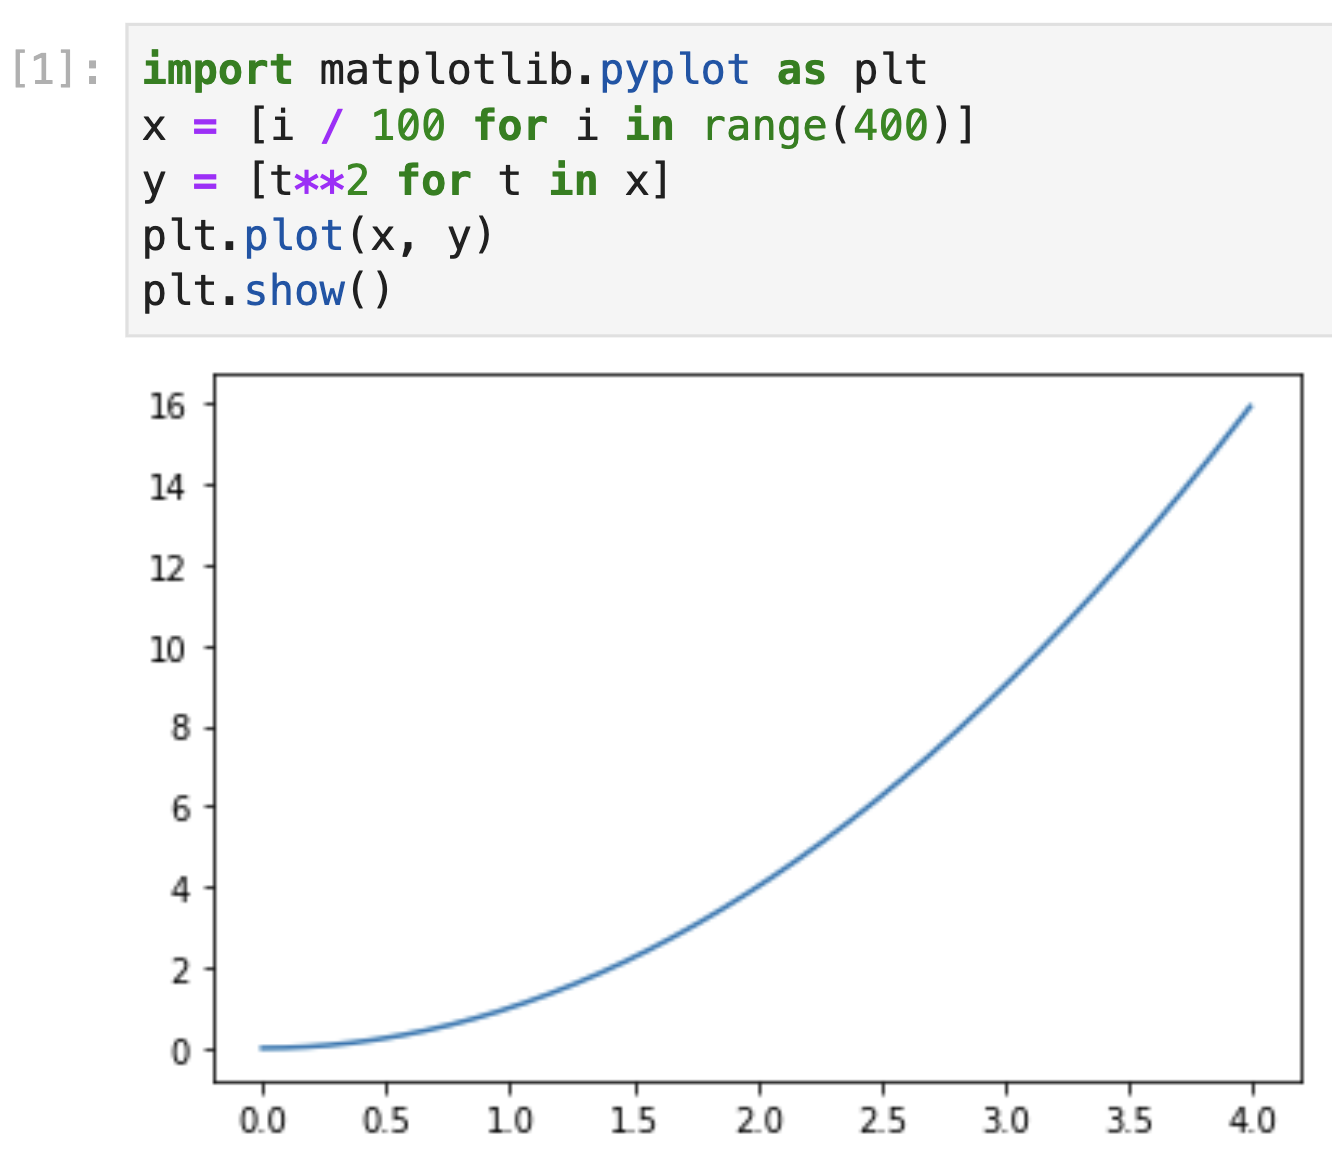
\includegraphics[width=0.9\linewidth]{work/example_matplotlib.png}
\caption{matplotlib でグラフを描画する例} \label{example_matplotlib}
\end{figure}

\subsection{SymPy}
SymPy は、記号計算のための Python ライブラリである。Symbol オブジェクトとして変数を作成し、Eq オブジェクトとして方程式を定義できる。subs 関数を使うことで、作成した方程式に数値を代入することができる。図~\ref{example_sympy} は、SymPy で Equation を定義し、数値を代入する例である。

\begin{figure}[bht]
\centering
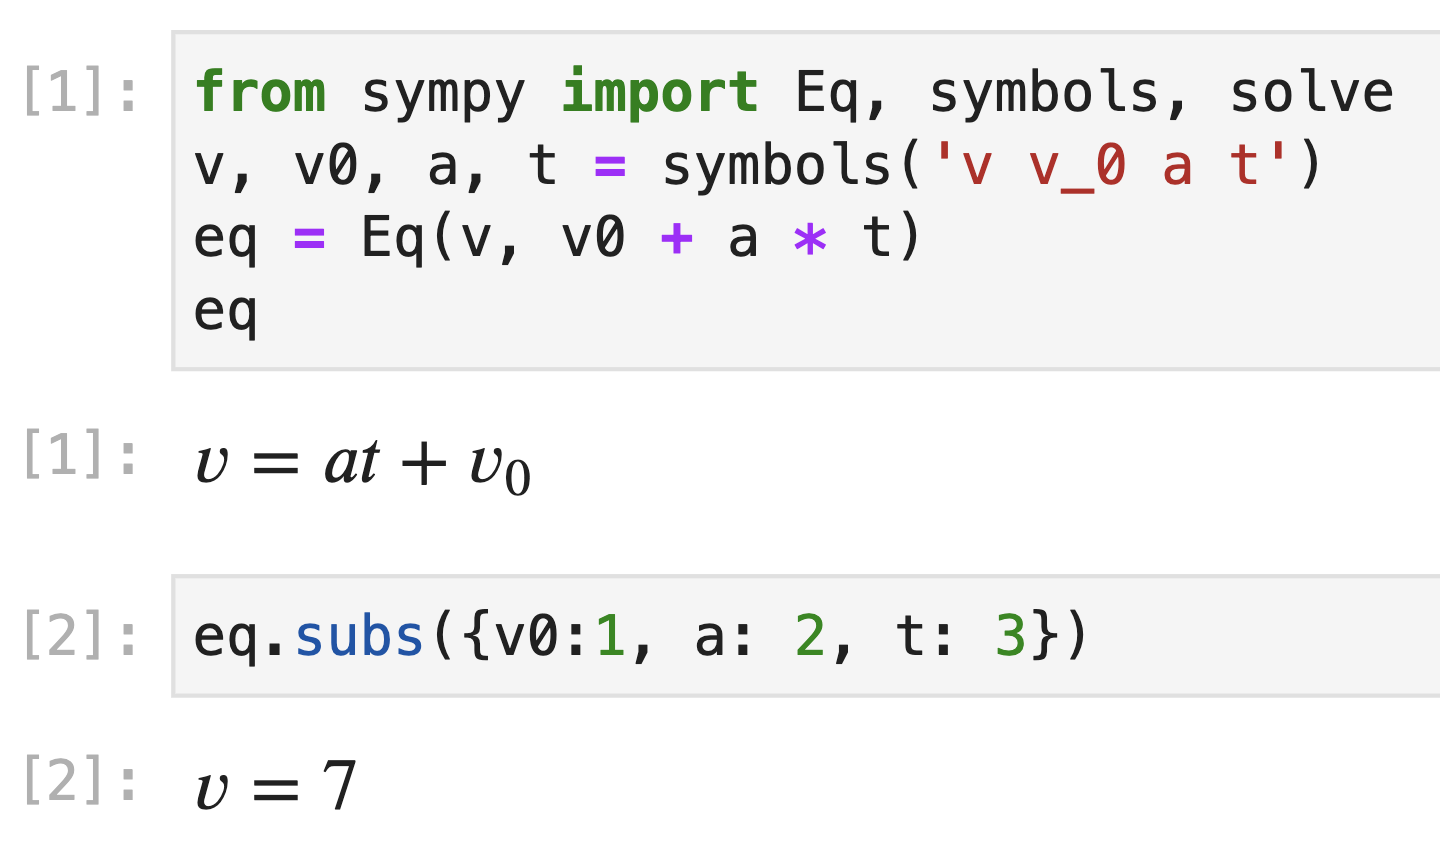
\includegraphics[width=0.9\linewidth]{work/example_sympy.png}
\caption{SymPy で Equation を定義し、数値を代入する例} \label{example_sympy}
\end{figure}

% 図~\ref{sympy_example}は、実際に SymPy で斜方投射を表す物理系を定義する例である。

% \begin{figure}[p]
% \centering
% 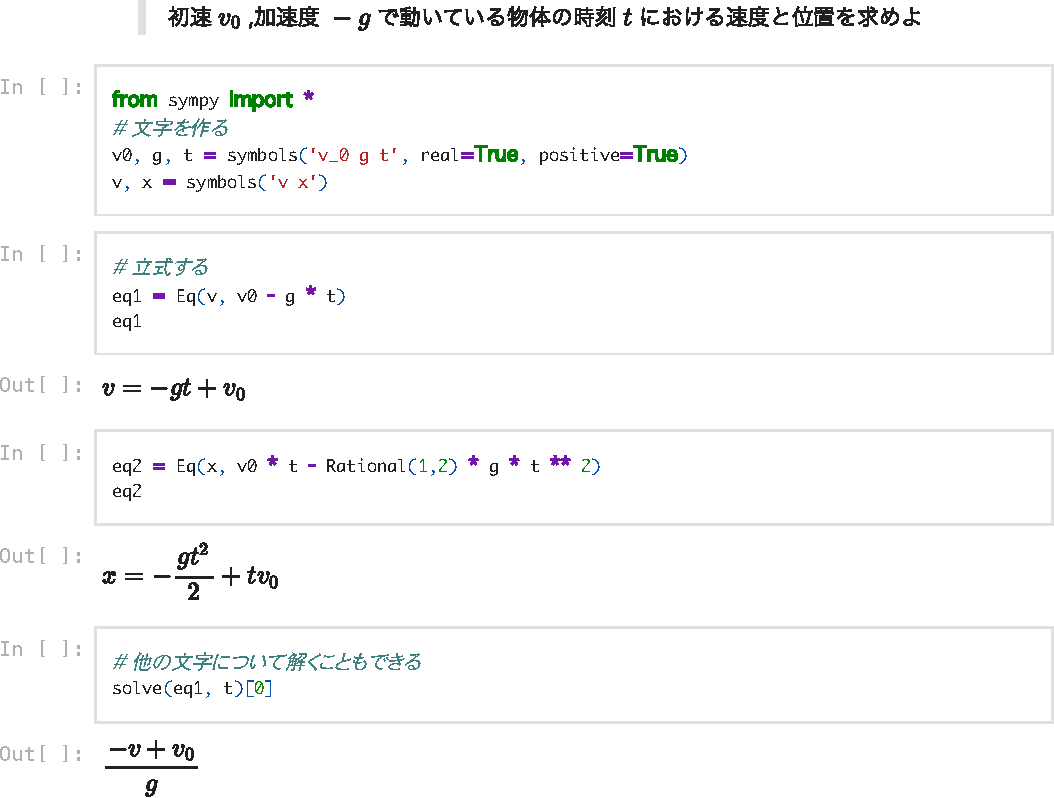
\includegraphics[width=\linewidth]{work/SymPy_example-crop.pdf}
% \caption{SymPy を用いて斜方投射を表す物理系を定義する例} \label{sympy_example}
% \end{figure}

% SymPy は次元を扱うことはできるのだが、次元が異なる値同士も足すことができてしまう。図~\ref{sympy_unit_example}では、$t$ に次元 $\mathrm{[T]}$ を、$g$ に次元 $\mathrm{[T/S^2]}$ を割り当てたが、$t + g$ が計算できてしまう。そのため、このような不一致を検出する仕組みを実装する必要がある。

% \begin{figure}[t]
% \centering
% 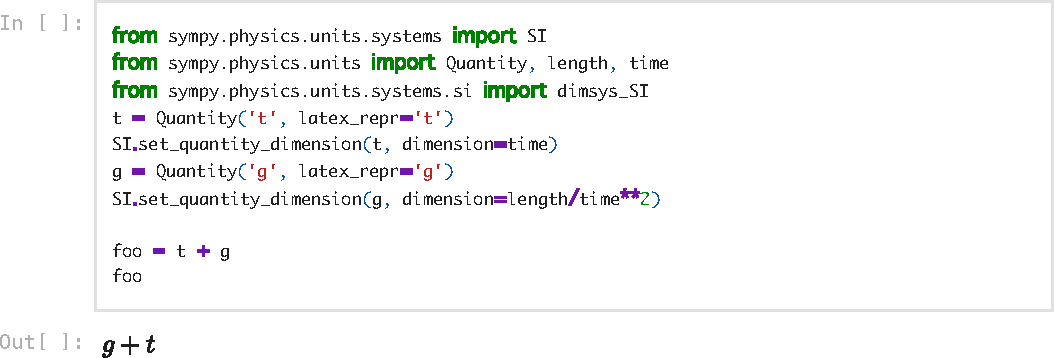
\includegraphics[width=\linewidth]{work/sympy_unit_example-crop.pdf}
% \caption{SymPy 上で単位が異なる値同士を足す例} \label{sympy_unit_example}
% \end{figure}

\newpage
\section{処理の流れ}
以下では、学習者の操作によって \simname がどのように物理系を定義しているかを簡単に説明する。

\begin{enumerate}
  \item 学習者が Jupyter 上の Widget に物体名を入力すると、\simname はその物体に紐づく変数を SymPy の Symbol として生成する。生成された変数は Jupyter 上に表示される。
  \item 学習者が物体と動作例を選択すると、\simname は動作例に応じた変数を Symbol として生成し、動作例の運動を表す Sympy の Equation を生成する。
  \item 生成された変数を利用した方程式を学習者が Jupyter 上の Widget に入力すると、\simname はそれを Equation として解釈する。またこの際、不正な次元の方程式になっていないかを確認する。 \label{未実装1}
  \item \simname は、選択された物体の座標・速度などを数値計算するために数値を与える必要のある変数を推論し、それらを入力するための Widget を生成する。 \label{未実装2}
  \item 学習者が数値を入力すると、Equation に数値が代入される。同時に動作例を表す Equation にも数値が代入され、matplotlib を用いて破線で描画される。
  \item 学習者が再生ボタンを押すと、時刻を表す変数 $t$ が時間変化し、物体の位置や座標が再計算され、matplotlib を用いて描画される。
\end{enumerate}

なおこれらのうち、\ref{未実装1}.に記した「学習者の入力を Equation として解釈する」「不正な次元の方程式になっていないかを確認する」、\ref{未実装2}.に記した「数値計算するために数値を与える必要のある変数を推論する」は未実装である。


% \section{lively.next}
% lively.next は Lively~\cite{ingalls_2008}から派生したプロジェクトで、ブラウザ上で GUI アプリケーションを作成・実行することができる Web プログラミング環境である。これを用いて、学習者が物体や方程式を定義する物理系定義ペインと、シミュレーション結果を表示する観測ペインを実装する。ブラウザ上で利用できるため、学習者はソフトウェアのインストールなどをする必要がなく、簡単に利用できる。

% \begin{figure}[hbt]
% \centering
% 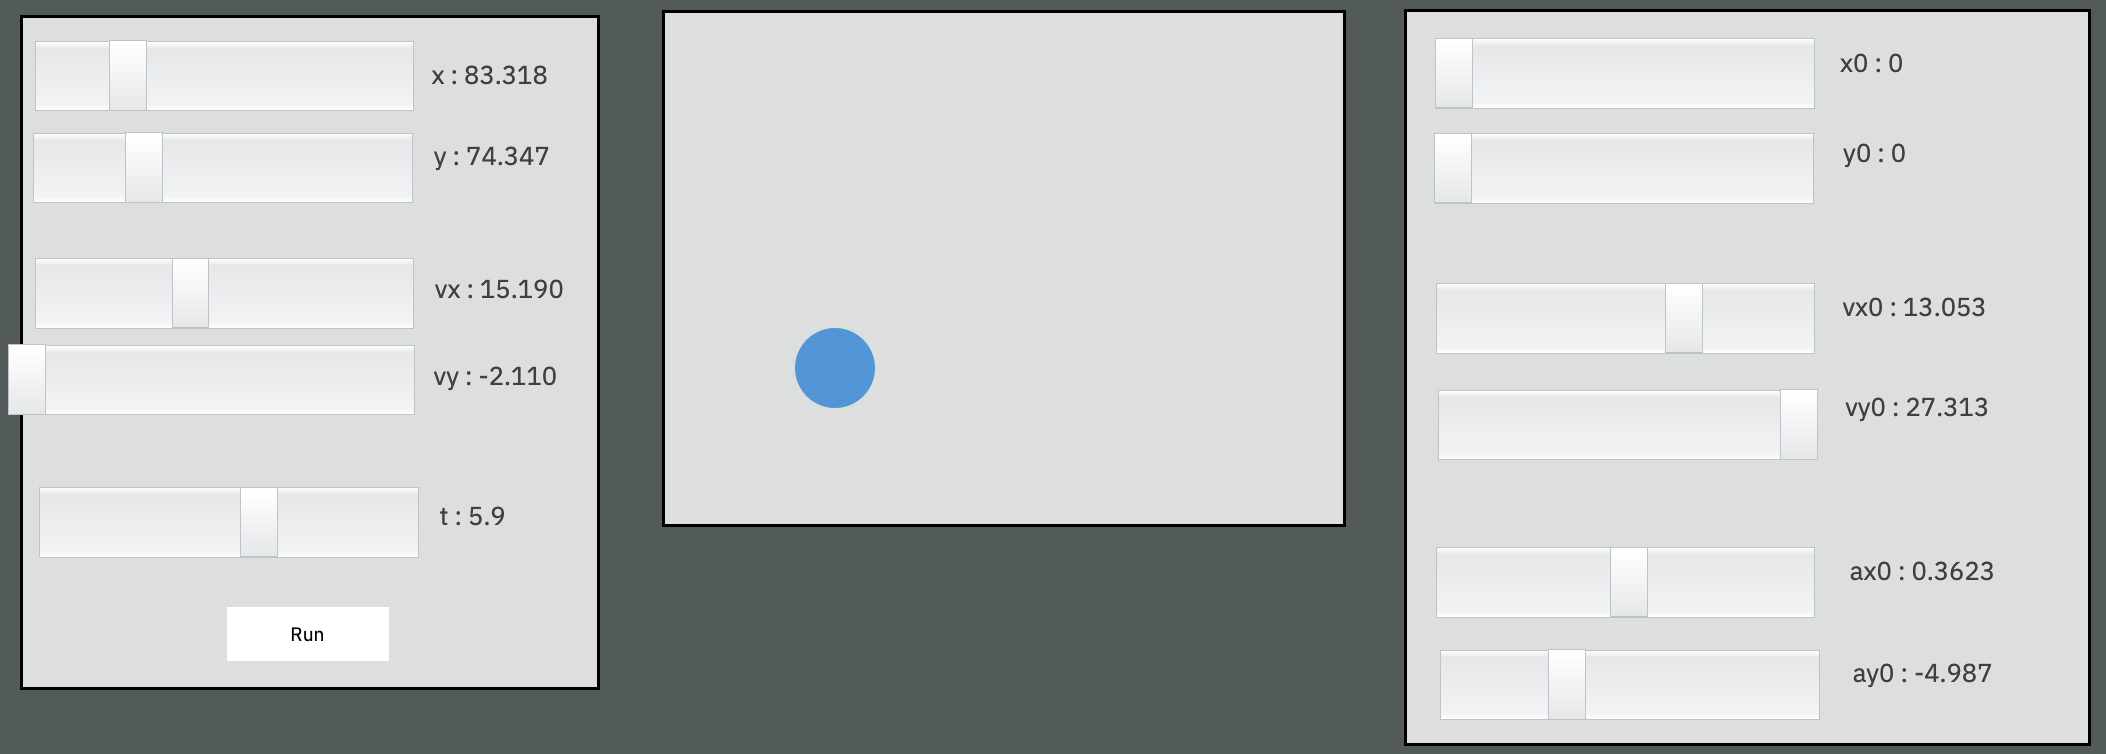
\includegraphics[width=0.9\linewidth]{figure/lively_example.png}
% \caption{lively.next を用いて実装されたシミュレーション結果の表示画面}
% \end{figure}

% SymPy は、記号計算のための Python ライブラリである。次元付き変数を作成し、方程式の処理や数値計算を行うことができる。図~\ref{sympy_example}は、実際に SymPy で斜方投射を表す物理系を定義する例である。

% \begin{figure}[p]
% \centering
% 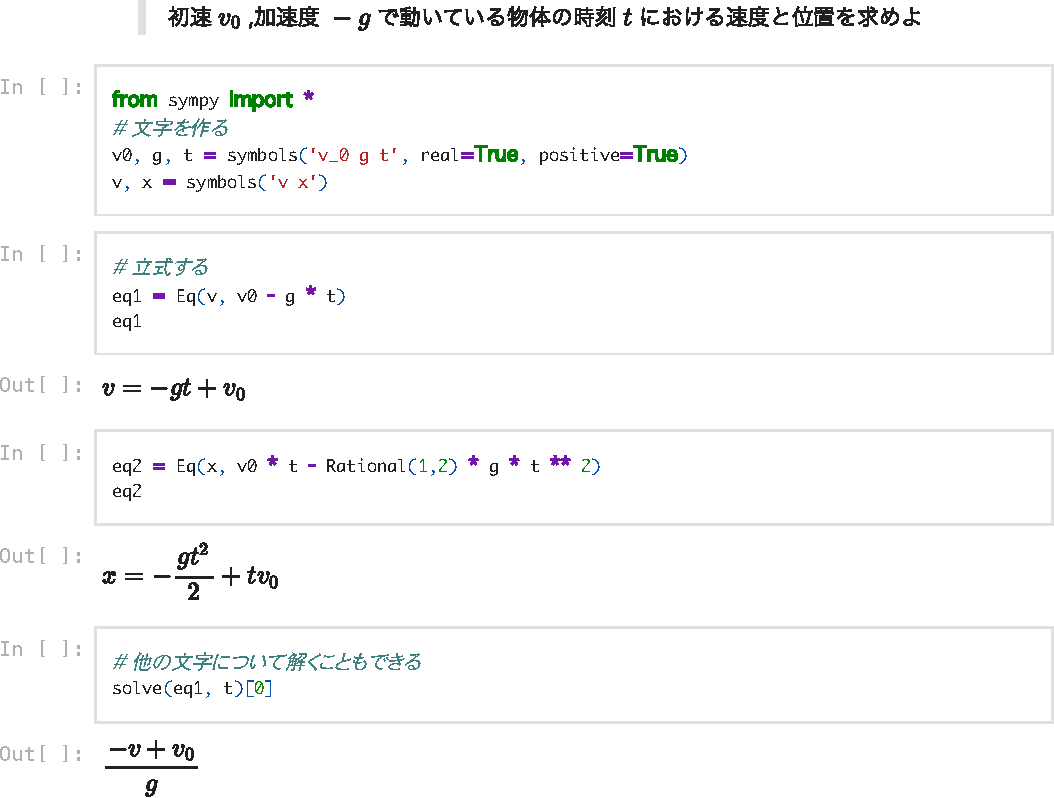
\includegraphics[width=\linewidth]{work/SymPy_example-crop.pdf}
% \caption{SymPy を用いて斜方投射を表す物理系を定義する例} \label{sympy_example}
% \end{figure}

% SymPy は次元を扱うことはできるのだが、次元が異なる値同士も足すことができてしまう。図~\ref{sympy_unit_example}では、$t$ に次元 $\mathrm{[T]}$ を、$g$ に次元 $\mathrm{[T/S^2]}$ を割り当てたが、$t + g$ が計算できてしまう。そのため、このような不一致を検出する仕組みを実装する必要がある。

% \begin{figure}[t]
% \centering
% 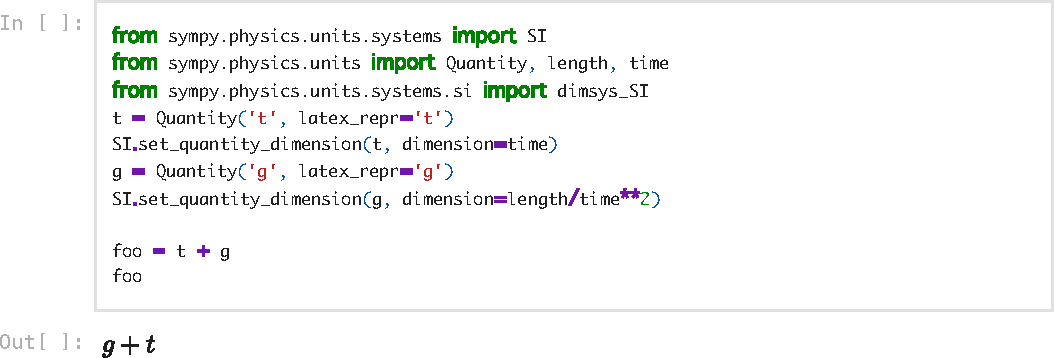
\includegraphics[width=\linewidth]{work/sympy_unit_example-crop.pdf}
% \caption{SymPy 上で単位が異なる値同士を足す例} \label{sympy_unit_example}
% \end{figure}

% また、SymPy は Python のライブラリであるが、後述する Pyodide を用いることでブラウザ上で実行することができる。

% \section{Pyodide}
% Pyodide は、Mozilla が開発している WebAssembly で実装された CPython 処理系である。ブラウザ上で Python コードを実行できる。また、Python で書かれたパッケージと C 言語で書かれた一部のパッケージに対応していて、SymPy は Pyodide で実行可能である。実際に Pyodide を実行する例を図~\ref{pyodide_example}に記す。

% \begin{figure}[htb]
% \centering
% \begin{lstlisting}[language=HTML]
% <!DOCTYPE HTML>
% <head>
%   <script src="https://cdn.jsdelivr.net/pyodide/v0.22.0/full/pyodide.js"></script>
%   <script>
%     async function main() {
%       let pyodide = await loadPyodide();
%       let result = pyodide.runPython(`
% import js
% result = js.document.getElementById("result")
% x = 2
% y = 10
% result.textContent += str(x ** y)
%       `);
%     }
%   </script>
% </head>
% <body>
%   <script>main()</script>
%   <p id="result">結果: </p>
% </body>
% \end{lstlisting}
% \includegraphics*{work/pyodide_example.png}
% \caption{Pyodide を利用する例} \label{pyodide_example}
% \end{figure}

% \section{シミュレーションの実行}

% シミュレーションの実行時は、設定された時刻 $t$ の範囲を粒度 $\Delta t$ ずつ変化させる。各方程式に各 $t$ を代入した結果を lively.next が受け取り、描画する。シミュレーションのリアルタイム性を確保するため、各 $t$ を方程式に代入した値は方程式の定義時・変数の値の変更時にあらかじめ計算する。

% \begin{figure}[hbt]
% \centering
% 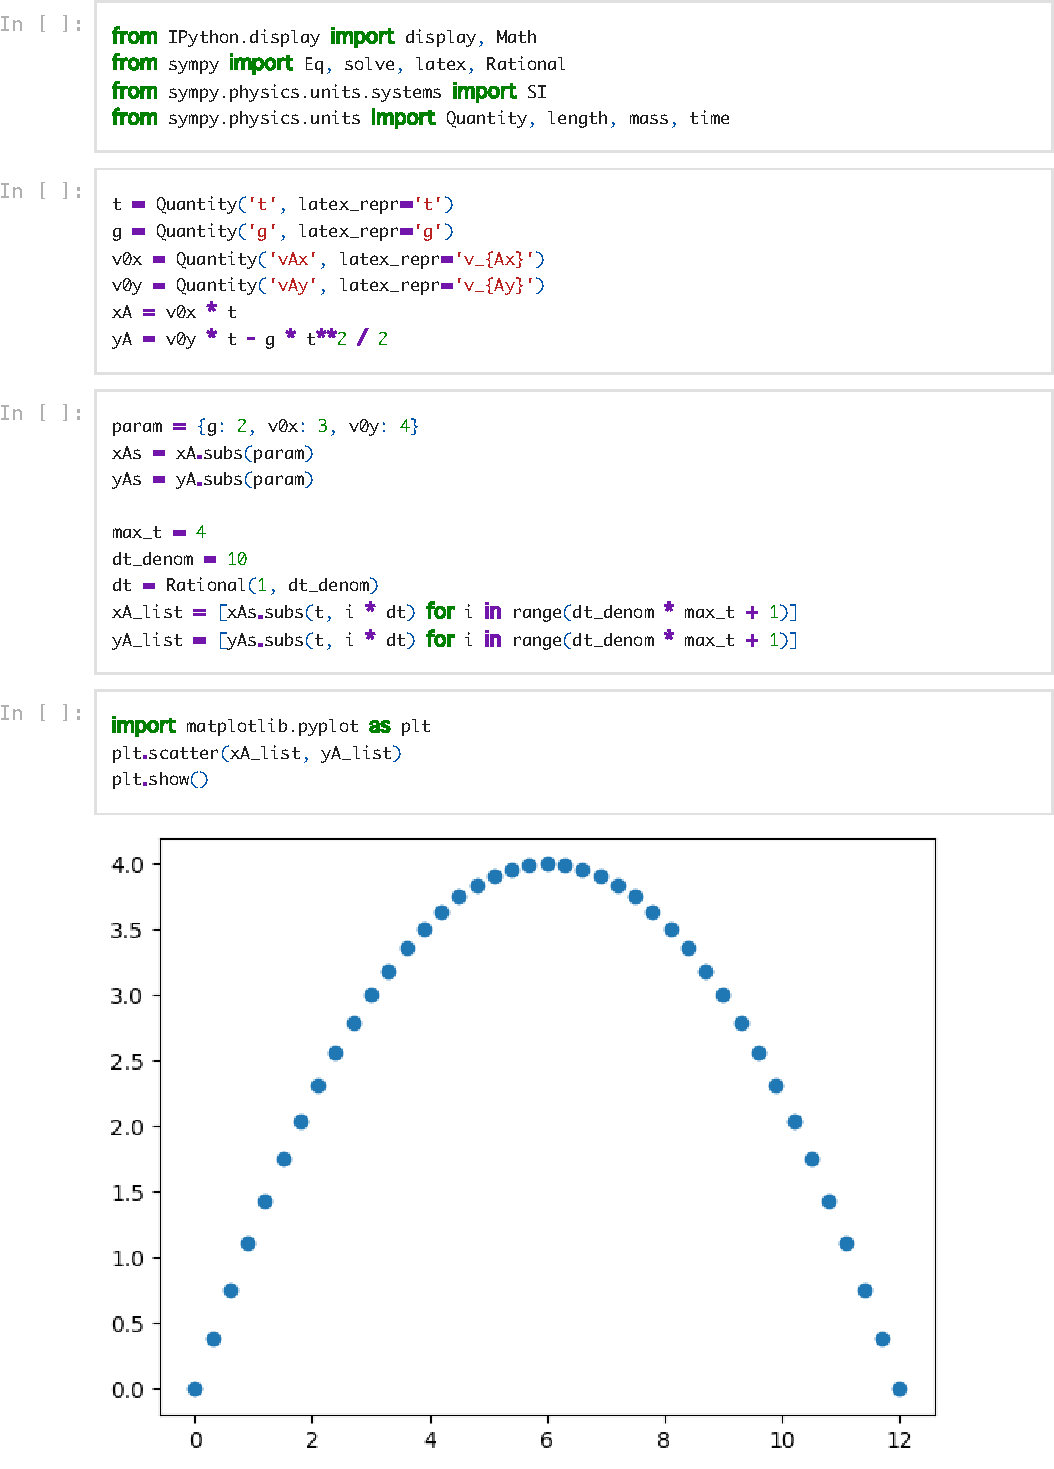
\includegraphics[width=0.85\linewidth]{work/deltat_example-crop.pdf}
% \caption{シミュレーション実行のための数値計算例} \label{deltat_exapmle}
% \end{figure}
